
%%%%%%%%%%%%%%%%%%%%%%%%%%% 1  %%%%%%%%%%%%%%%%%%%%%%%%%%%
\section{An 8 x times,5 Gb/s Parallel Receiver With Collaborative Timing Recovery \cite{agrawal20098}}  \label{ss:agrawal20098}
%%%%%%%%%%%%%%%%%%%%%%%%%%% 1  %%%%%%%%%%%%%%%%%%%%%%%%%%%

Clock frequencies have been increasing in the early part of the century up to a certain point.
To alleviate bottle-necks in the performance of a system the \textit{off-chip} input and output (I/O) should also be scaled.
Scaling of \acc{bw} is obviously achievable by implementation of parallel I/O.
Digital systems need a clock signal for operation.
Nowadays, digital systems are relatively large \footnote{more parallel I/O leads to a larger system.} and this gives problems in synchronicity of digital systems.
To correct for this, timing recovery (or symbol synchronization \cite{mueller1976timing}) is applied.
Parallel links are conventionally implemented as \acc{embeddedlink} (see: \cref{fig:rep1:seriallinks}) or as \acc{synclink}  (see: \cref{fig:rep1:synclinks}).

\begin{figure}	\centering
	
	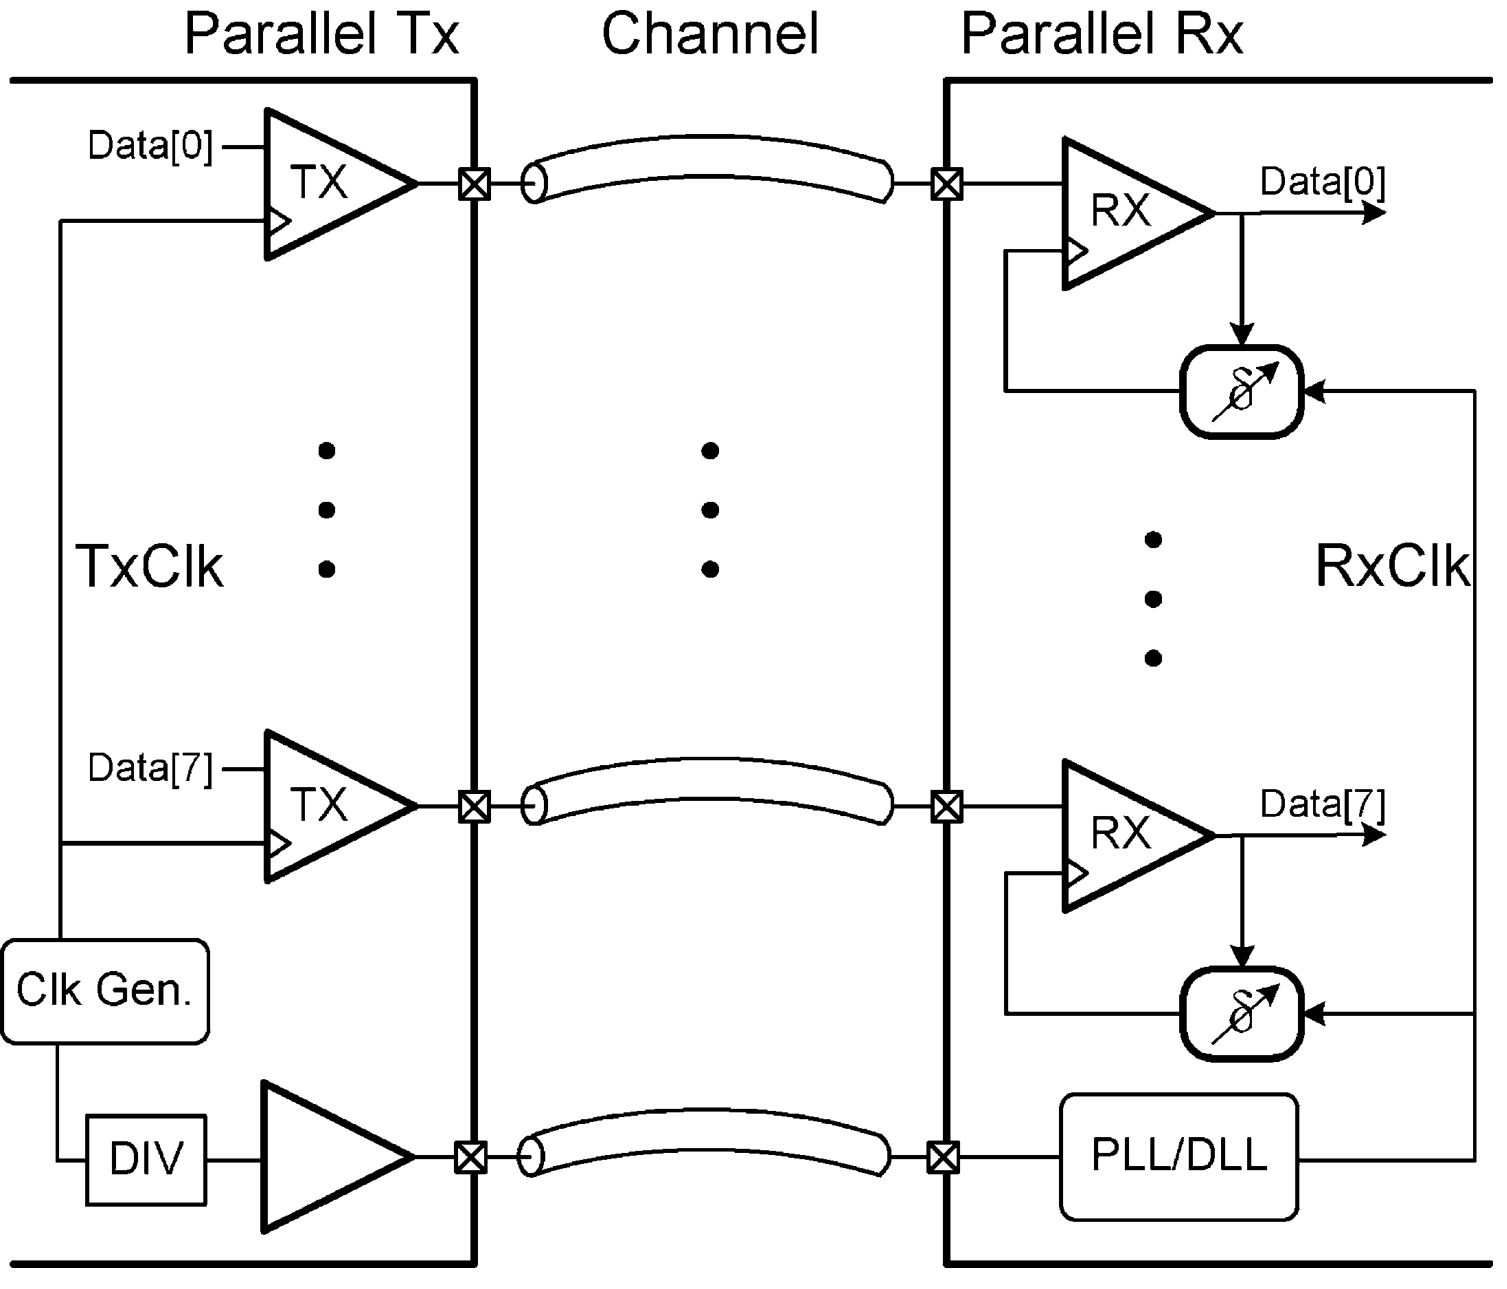
\includegraphics[width=0.8\linewidth]{Figures/Rep1SourceSync.png}
	\caption{Ensemble of serial links (\textit{embedded clock link}) (\ac{embeddedlink}), Source: \cite{agrawal20098}.} 
    \label{fig:rep1:seriallinks}
\end{figure}

\begin{figure}	
    \centering
	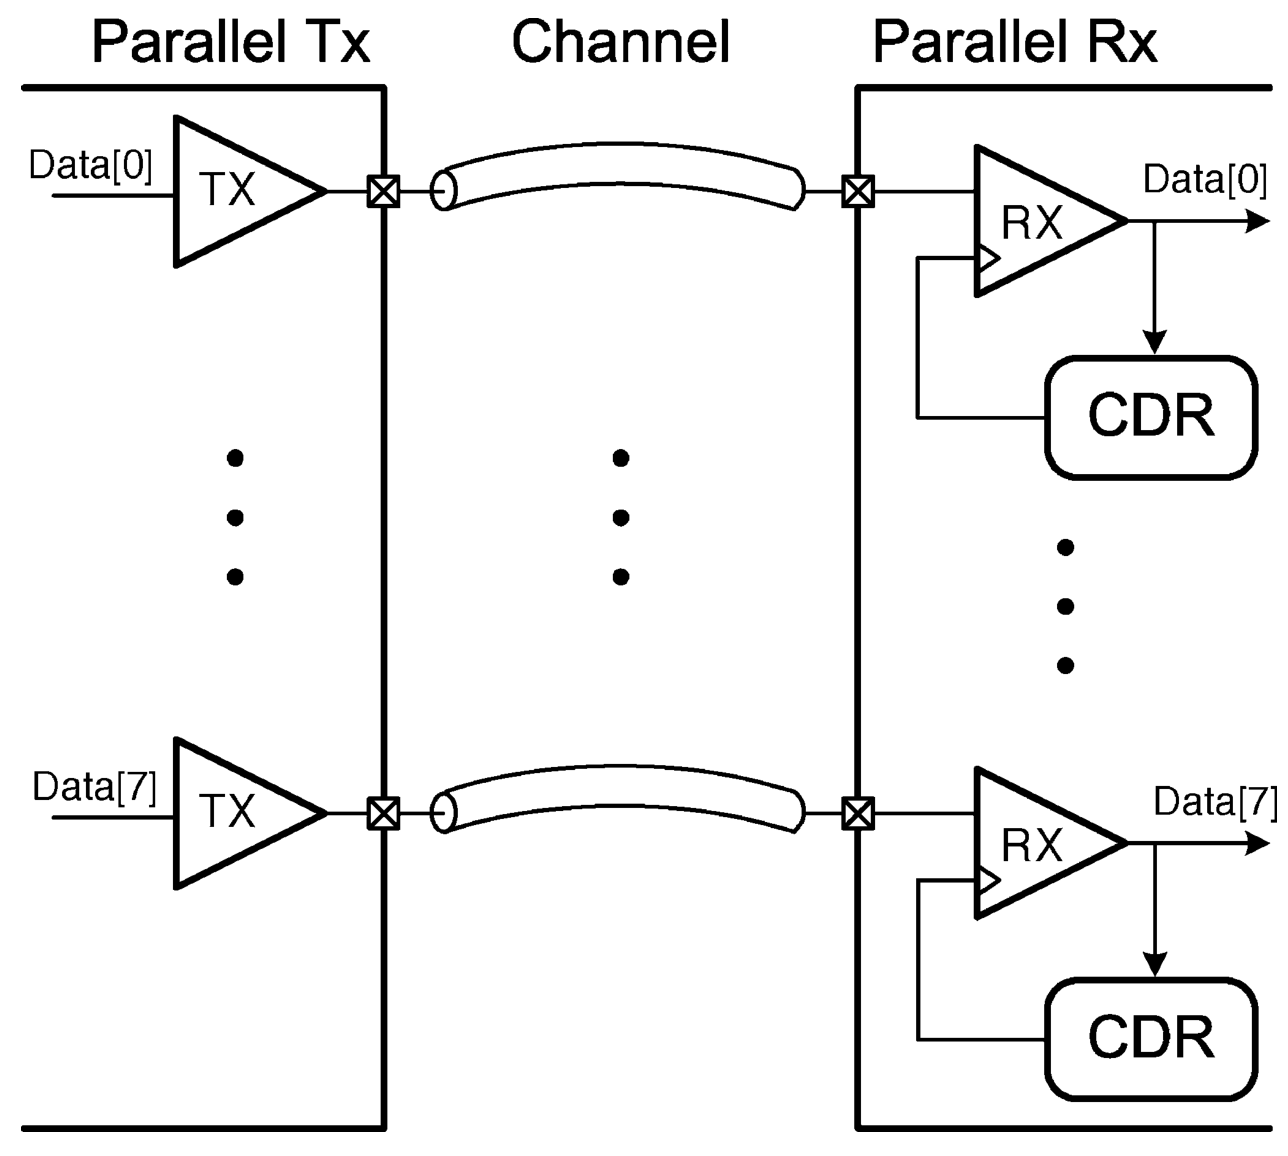
\includegraphics[width=0.8\linewidth]{Figures/Rep1EnsembleSerLinks.png}
	\caption{Source-synchronous links (\textit{forwarded-clock link}) (\ac{synclink}), Source: \cite{agrawal20098}.} 
    \label{fig:rep1:synclinks}
\end{figure}

In \ac{embeddedlink} the receiver extracts the clock from the data, as it is embedded in the data. 
In \ac{synclink} a clock line is sent along the data and the receivers can use it for timing recovery. 
\objective
The increased I/O \ac{bw} puts a strain on the latency, power consumption and form-factor requirements and causes jitter amplication. 
\motive
The research aim of this paper is to merge the desirable characteristics of both \ac{embeddedlink} as \ac{synclink} into \acc{coltimrec}.
This design comes with an power and area overhead of 10-15\% relative to \ac{synclink} but is more efficient than the \ac{embeddedlink} and also increases the effective edge transition density.
% \footnote{This concept is more clearly explained in \cite{miller2005transition}}.
\summary
The design of the \ac{coltimrec} is shown in \cref{fig:rep1:coltimrec}. 
It does not contain a clock link (as in \ac{synclink}) and instead of a local \acc{cdr} as seen in \cref{fig:rep1:seriallinks} the local clock data is connected to a \acl{gtr} block (\ac{gtr}) which carries the responsibility of the providing the global clock.

\begin{figure}
    \centering
	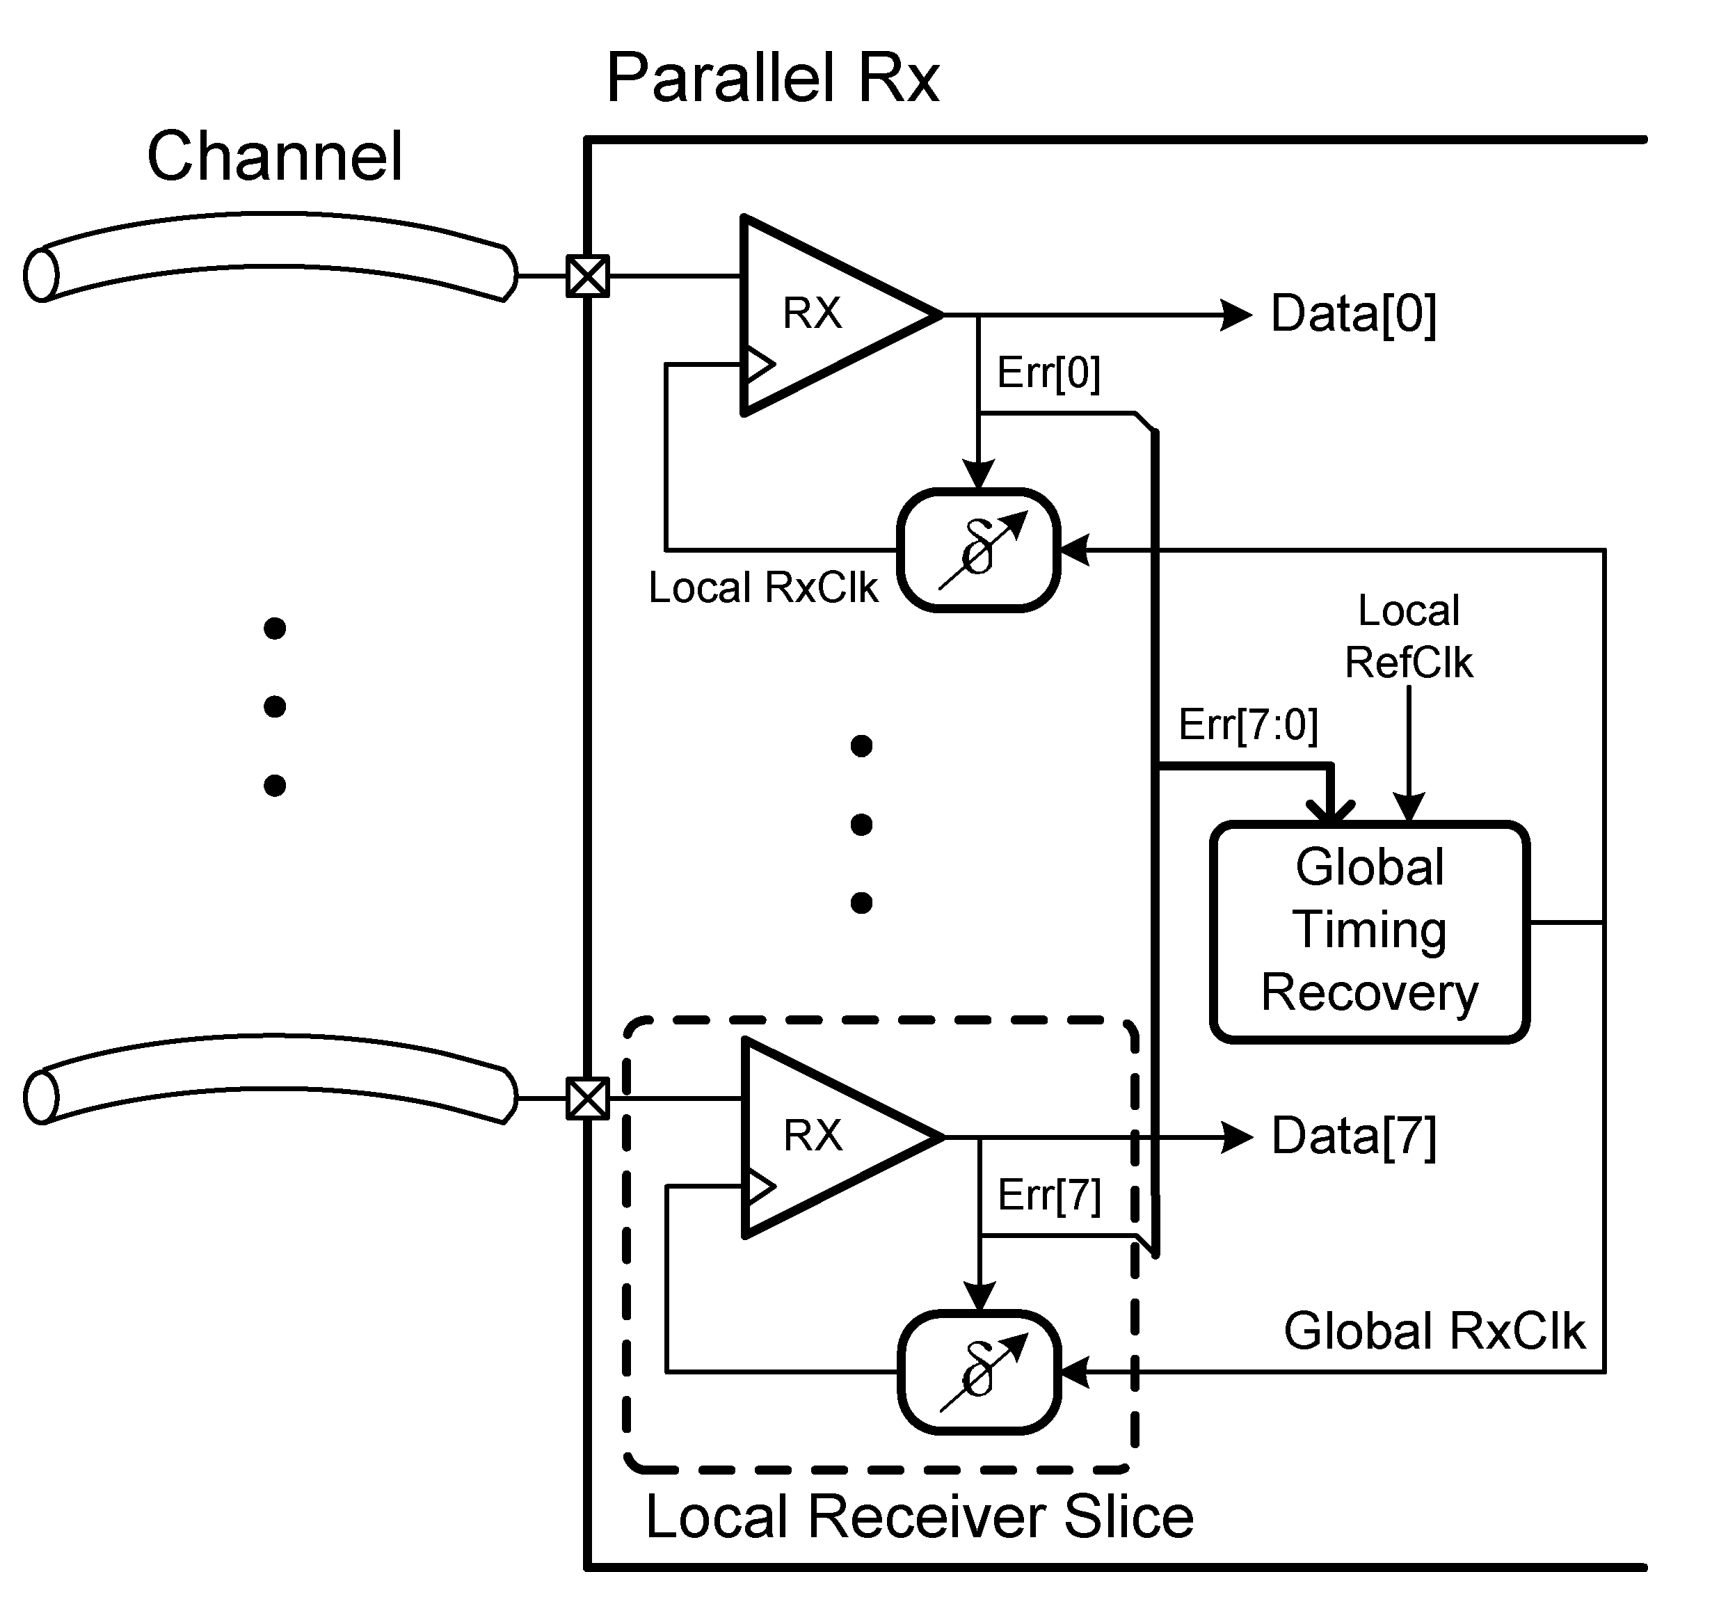
\includegraphics[width=0.85\linewidth]{Figures/Rep1CombLink.png}
	\caption{\acc{coltimrec}, Source: \cite{agrawal20098}.} 
    \label{fig:rep1:coltimrec}
\end{figure}

A comparison has been made between three different levels of jitter scenarios regarding phase-tracking error for each system (\ac{embeddedlink}, \ac{synclink} and \ac{coltimrec}). %\footnote{Jitter: the deviation from periodicity, it is a form of noise. Dither on the other hand is intentional noise in an out of band frequency.} 
The noise levels are devided in the following way: low-frequency jitter (around 1 MHz), midfrequency jitter (around 30 MHz) and high-frequency jitter (around 1 GHz).
Phase tracking at low-frequency jitter is best for \ac{embeddedlink}. 
At mid-frequency jitter the \ac{coltimrec} behaves much better than the other implementations. 
At high-frequency jitter all systems behave poorly.
However, trends show that mid-frequency jitter is growing, which motivates \ac{coltimrec}.

The design of the \ac{coltimrec} (\cref{fig:rep1:coltimrec}) consist of two global parts: the phase adjustment element and the \acc{gtr} block.
Each local receiver sends early/late timing information to the \ac{gtr}.
The \ac{gtr} sends the recovered clock (Global RxClk) that tracks the frequency and the jitter of the data signals.
% \footnote{Skew: the possible difference in arrival time of the clock in different sections of a design} 
To handle the interchannel skew the local receivers alter the phase of the Global RxClk for inter-channel skew.

% Explain the GLOBAL working of the global timing recovery circuit
The \ac{gtr} is comprised of an Error retimer, phase error summer, $2^{nd}$ order filter, \acc{pll} and a phase interpolator.
The error retimer aligns the clock of 8 channels to a reference clock.
The phase error summer, sums the phase error of the 8 channels and passes it to the filter.
The filter delivers the decoded information to the \ac{pll} and the phase interpolator.
The \ac{pll} receives the filter information and uses it to select odd and even phase difference (2 4b-muxes).
This is coarse grained phase generation.
The phase interpolator provides a 256 phase steps per clock period delivery (more fine grained phase adjustment).
% Explain the GLOBAL working of the phase adjustment element
The phase adjustment consists of two \accs{dll}, data sampler (8 channels), duty-cycle corrector, skew-compensation element and a phase spacing error correction circuit (see: \cref{fig:rep1:receiver}).
The global clock (from the \ac{gtr}) is corrected for its duty-cycle.
The first \ac{dll} provides phase de-skewing for phase alignment of its local clock and the data.
The second \ac{dll} generates 8 uniformly spaced clock phases to drive the interleaved data samplers.
%not clear why
Reasons for using the cascaded \acsp{dll} approach are: \acsp{dll} do not limit the global TR \ac{bw} and they require only one phase to generate a local clock.
However, the two \acsp{dll} could be replaced by one \ac{pll}.
This was not applied because \acsp{dll} do not apply phase filtering. 
But there are disadvantages to \acsp{dll} that should taken into account.
For instance, \acsp{dll} are very sensitive to the duty cycle of the reference clock and the shape of the reference clock can amplify a mismatch in phase spacing.

\begin{figure}	
    \centering
	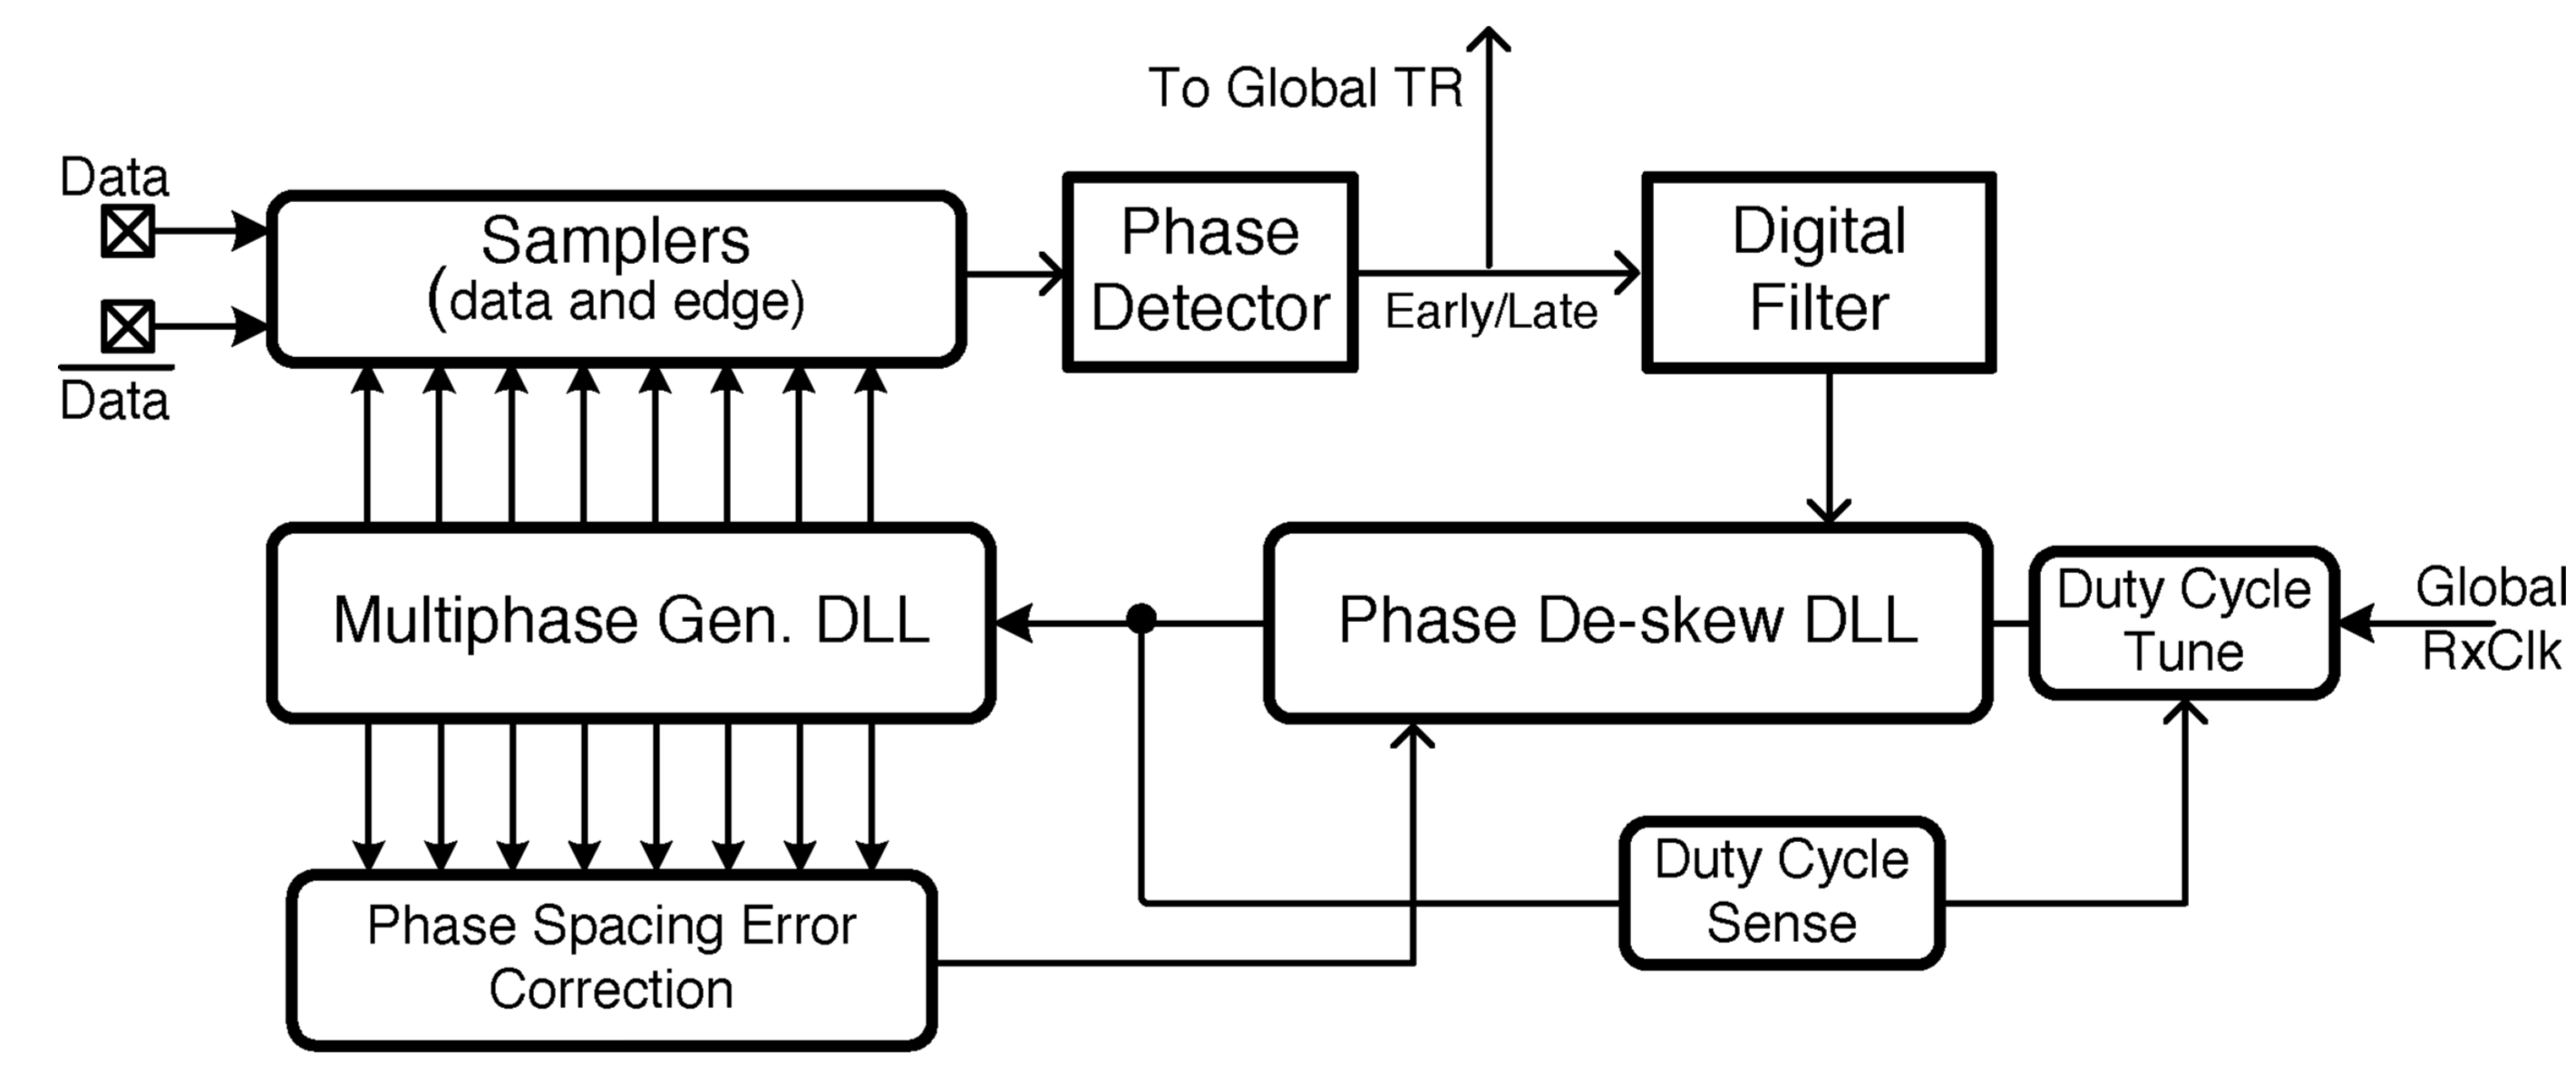
\includegraphics[width=0.99\linewidth]{Figures/Rep1ReceiverSlice.png}
	\caption{Local receiver slice block diagram, Source: \cite{agrawal20098}.} 
    \label{fig:rep1:receiver}
\end{figure}
% Measurements and results
The setup was tested on 130 nm CMOS logic. 
To test the chip 8 synchronous PRBS data signals are needed which also add amounts of correlated jitter.
This was done by using a Tektronix 5334 up to 3.2 Gb/s.
For the higher rates an FPGA based parallel transmitter was used.
Not all channels were tested due to restricted connector spacing on the board .

\Cref{fig:rep1:result} shows the dithering jitter on the recovered clock. 
When the number of channels share timing information the dithering jitter reduces from 2.7ps to 2.2ps.

% Discussion / conlusion
Wideband jitter tracking, by reducing dithering jitter on the received clock, is possible when implementing \ac{coltimrec} however there is an area and power overhead (respectively 8.5\% and 15\% per receiver).

\begin{figure}	\centering
	
	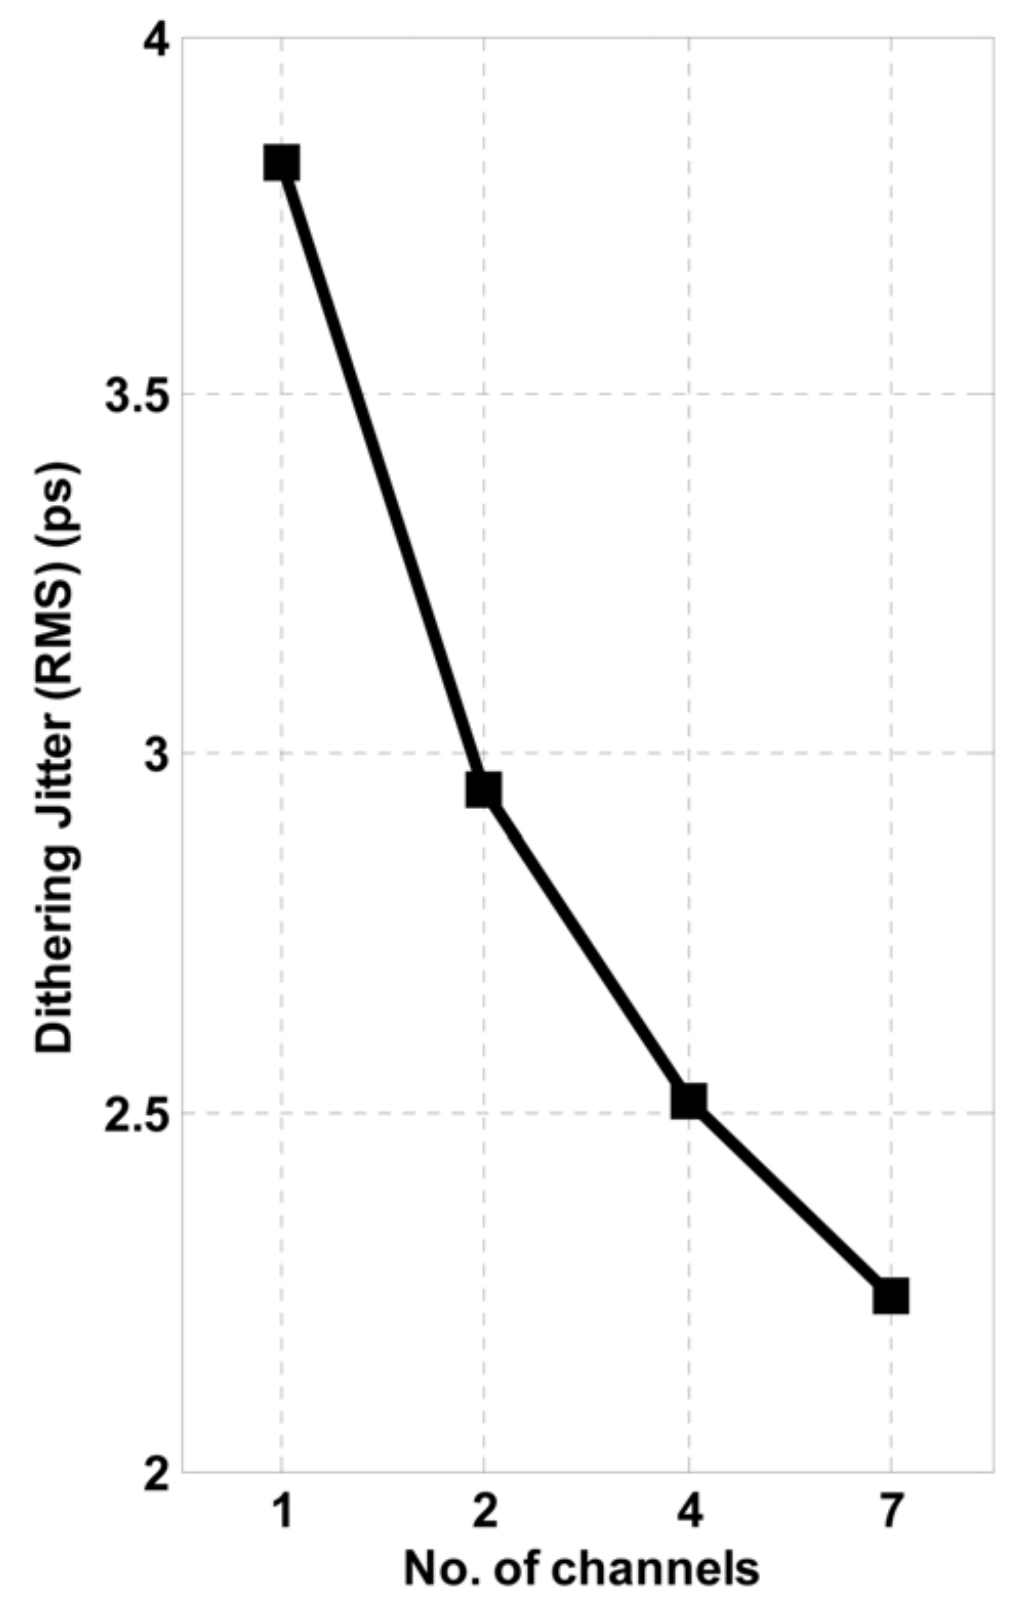
\includegraphics[width=0.7\linewidth]{Figures/Rep1Result.png}
	\caption{Measured RMS jitter for different degrees of collaboration, Source: \cite{agrawal20098}.} 
    \label{fig:rep1:result}
\end{figure}

% Motive: Statement indicating why the research was done (e.g. a gap in
% knowledge, contradictory results). The motive leads to the objective.
% • Objective: Statement about what the authors want to know. The
% objective may be formulated as a research question, a research aim, or a
% hypothesis that needs to be tested.
% • Main conclusion: Statement about the main outcome of the research. The
% main conclusion is closely connected to the objective. It answers the
% research question, it says whether the research aim was achieved, or it
% states whether the hypothesis was supported by evidence.

% In the body, you should:
% - Group research studies and other types of literature (reviews, theoretical articles, case studies, etc.) according to common denominators such as qualitative versus quantitative approaches, conclusions of authors, specific purpose or objective, chronology, etc.
% - Summarize individual studies or articles with as much or as little detail as each merits according to its comparative importance in the literature, remembering that space (length) denotes significance.
% - Provide the reader with strong "umbrella" sentences at beginnings of paragraphs, "signposts" throughout, and brief "so what" summary sentences at intermediate points in the review to aid in understanding comparisons and analyses.


